\chapter{Planteamiento Metodológico}

Para la metodología se optó por el campo computacional usando softwares especializados en lo que es interacciones y dinámicas moleculares

\section{Lugar en donde se desarrollará la investigación}
El lugar donde se desarrollará esta investigación es en Centro de Investigación en Ingeniería Molecular (CIIM) autorizado y supervisado por el Dr. Badhin Gómez Valdez   

\section{Ambientes por utilizar}
Se usaran los ambientes asociados al centro de investigación cuya estación de trabajo está preparada y optimizada para generar los resultados esperados dentro de la preparación, dinámica y análisis molecular. 

\section{Materiales}
Para esta investigación se han de requerir computadores óptimos para los cálculos cuánticos que se tienen que llevar a cabo:

\subsection{Hardware}
\begin{itemize}
    \item Procesador AMD Ryzen 9 
    \item Placa madre X570 gaming
    \item GPUs NVIDIA 3080 y NVIDIA 2080
    \item sistemas de ventilación optimizados
    \item Fuente de poder de Seasonic 80 Plus Gold
\end{itemize}

\subsection{Software}
\begin{itemize}
    \item Sistema operativo Linux 24.04
    \item Chimera X
    \item AlphaFold3 (Nativo)
    \item Autodock Vina (Nativo)
    \item Gromacs v.2024.3 
    \item Gaussian y derivados
\end{itemize}

\section{Métodos}

\subsection{Interacción proteica en estado basal de la enzima DPP4}
Para ello haremos uso de los softwares de predicción de modelos proteicos como lo es el modeller integrado en el software Chimera X al igual que AlphaFold3 que tienen la finalidad de predecir el estado de la proteína por comparación.

El primero objetivo a cumplir es la extracción de la proteína de una base de datos como lo es Protein Data Bank (PDB) luego de encontrar la enzima adecuada verificando la mejor valoración según bibliografía procedemos a realizar la construcción de la molécula si lo necesita, posterior a ello procedemos a la búsqueda de la proteína blanco como lo es el Péptido Parecido al Glucagón (GLP1) de la misma forma valoramos por búsqueda bibliográfica los estadios de la molécula y usamos softwares de modelado si esto lo requiere, Softwares como AlphaFold que mejora considerablemente al tenerlo integrado a la máquina donde se trabajará el modelado de las proteínas.

Después de haber realizado la limpieza de las proteínas y completado todos los residuos a utilizar si estos lo requieren. Generamos dinámicas moleculares usando GROMACS como software y OPLS como campo de fuerza a las proteínas por separado, esto con el fin de estabilizar ambas proteínas y encontrar su estado basal independiente gracias a los gráficos de dinámica.
Posterior a ello procederemos a la interacción proteica esto se realizará con un dockeo a nivel citoplasmático como es normalmente, en este caso mantenemos la GLP1 estable mientras que la enzima dse aproxima como ligando, normalmente mientras más veces repita el Autodock vina presenta mejor probabilidad estadística de brindar un resultado estable donde podemos afirmar el valor inhibitorio en estado basal de ambas moléculas cuando interaccionan en el estado de catálisis enzimática.

\subsection{Generación de la base de datos de ligandos}
Para este punto se requiere del análisis de bibliografía especializada en ligandos de interés como pueden ser ligandos encontrados en el Aloe Vera con aplicaciones antidiabéticas pero también los ligandos encontrados para otras funciones podrían ser resultados favorables es por ello que hacemos una búsqueda de aproximadamente 113 metabolitos gracias a diferentes bases de datos los cuales serán filtrados por bibliografía y por el estándar ADMET que nos ayudará a buscar los mejores resultados para tener valores altos de druagabilidad protética y así generar la inhibición de DPP4.

Finalmente usaremos la base de datos de estudios previos farmacológicos que nos agreguen la mayor cantidad de fármacos comerciales sintetizados con la finalidad de generar la inhibición de DPP4. Estos fármacos presentan a la familia de las gliptinas como una de las más importantes pero se agregarán muchos mas dependiendo del análisis bibliográfico y el filtro ADMET que nos ayudará a buscar estadísticamente los mejores resultados para la interacción como ligandos inhibidores de la actividad enzimática de la DPP4. 

\subsection{Análisis de resultados por dinámica molecular y análisis estadístico}
Dependiendo de los resultados generaremos un análisis de los mejores ligandos tanto de los ligandos sintéticos como de los de procedencia natural ya que la liste ha reducido considerablemente se pude realizar un ultimo dockeo con el fin de encontrar diferencias en las energías de interacción ya que de esta evaluación se generará un análisis estadístico para evidenciar los mejores ligandos con mejor potencial inhibitorio decidiendo finalmente si los metabolitos extraídos del aloe vera podrían superar la inhibición de los actuales fármacos usados para el tratamiento de la Diabetes Mellitus Tipo 2.

\section{Flujograma de actividades }

%\begin{figure}
 %   \centering
 %   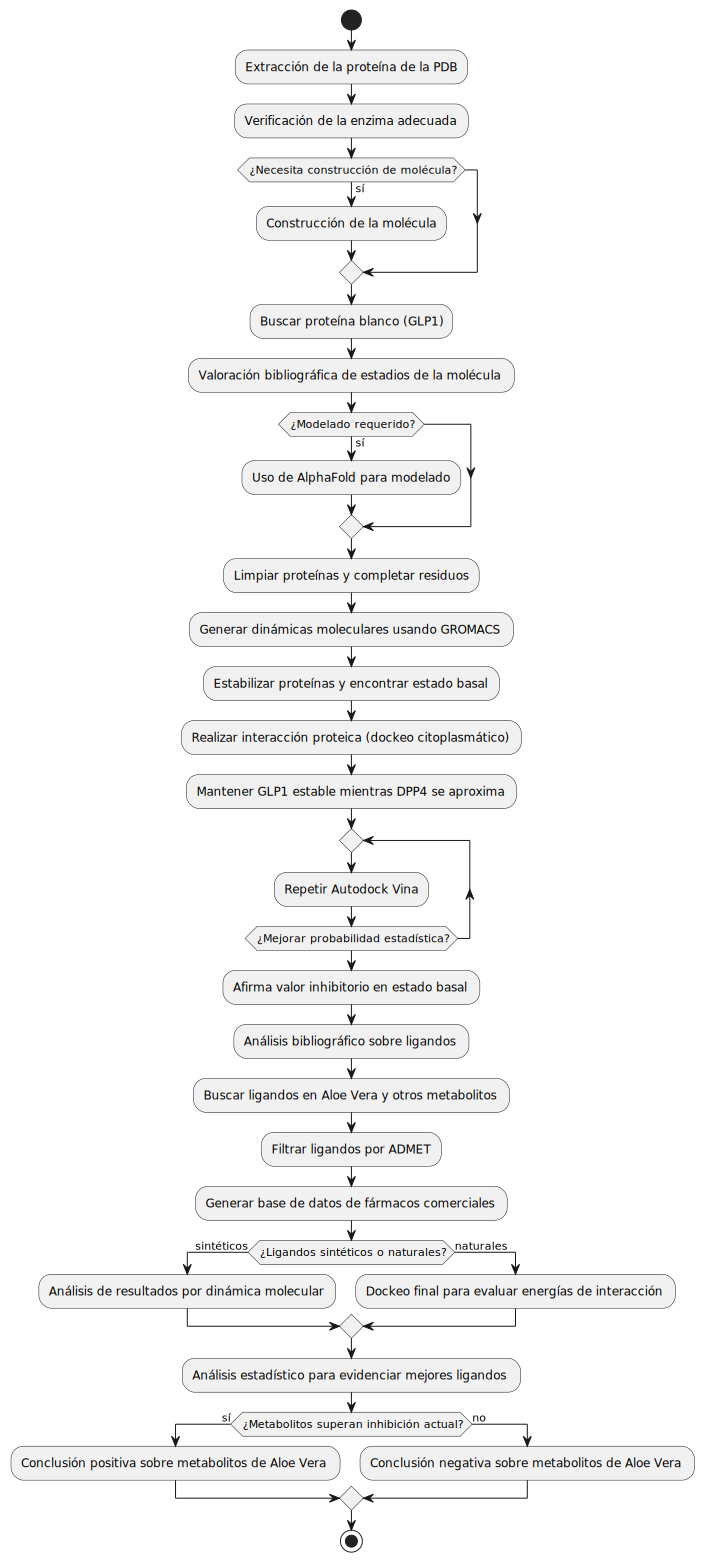
\includegraphics{figuras/Flujograma.svg}
 %   \caption{Figura}
 %   \label{Flujograma}
%\end{figure}



